\documentclass[a4paper,12pt]{article}

\usepackage[left=2.5cm, right=2.5cm, top=3cm, bottom=3cm]{geometry}

\usepackage{amsmath, amsthm, amssymb}

\usepackage[spanish]{babel}

\usepackage{cite}

\usepackage{graphicx}

\usepackage{url}

\bibliographystyle{apalike}

\begin{document}
\title{Proyecto de Ciencia de Datos}
\author{Javier Pérez Montero}
\date{Julio, 2023}
\maketitle


\begin{abstract}
    En este proyecto presentamos el análisis detallado de algunos productos del día a día. 
    Presentamos paso a paso todo el procedimiento que se llevó a cabo para la elaboración de dicho proyecto. 
    El proyecto tiene su base en el esfuerzo de presentar cada uno de los datos con la mayor cautela y detalle, yendo a la raíz de la información. 
    Se visitaron cafeterías y agros al 100 por ciento para obtener la mayor veracidad de la base de datos que presentaremos a continuación.


\end{abstract}

\section{Introducción}\label{sec:intro}

En esta ocasión, escogimos 4 productos para trabajar y analizar su comportamiento conforme a la situación actual. 
Dichos productos son: cerveza, cebolla, refresco instantáneo y refresco gaseado. 
Conforman el análisis de dicho proyecto. 
Estaremos respondiendo varias preguntas que surgieron a medida que trabajábamos. 
Junto con relaciones, comparaciones y, sobre todo, fomentar como objetivo la investigación de cada producto.

\section{Códigos de Importación y Bibliotecas}\label{sec:ent}
Para la confección de nuestra base de Datos utilizamos un archivo tipo(.json) en el cual se detalla en cada línea las categorías de datos que recolectamos de los productos antes dicho. 

  Para poderle dar una mejor presentación de una forma más interactiva y menos tediosa de visualizar, decidimos presentar la información en varias gráficas y tablas explicativas, estas fueron importadas de varias bibliotecas que utilizamos.
  Como:
\begin{itemize}
    \item Pandas
    \item Matplotlib
    \item Numpy
    \item Seaborn
    \item Plotly
    \item Folium
\end{itemize}

\section{Recolección y Recopilación de Datos}\label{sec:ent}
Como explicamos anteriormente, nos tomamos la molestia de realizar trabajo de campo y hacer una recolección exhaustiva pero muy beneficiosa para presentar una información veraz. 
Utilizando Pandas, una de las bibliotecas que mencionamos antes, presentaremos en las siguientes celdas los códigos para realizar las tablas en donde se ilustran los datos de cada uno de los productos de nuestro archivo .json.

En nuestro proyecto, recopilamos datos con respecto a la ubicación e imágenes de cada uno de los lugares que visitamos en el municipio de Marianao, el municipio experimento de nuestro proyecto. 
Las imágenes se encuentran como prueba de la recopilación de los datos y se habilitó una carpeta donde se pueden ver cada una de ellas, en caso de ser necesario. 
A medida que avancemos en la presentación, podrás acceder a distintas imágenes para una mejor visualización del contenido. 
La geolocalización es característica en nuestros datos, ya que se puede presenciar el lugar exacto de donde se extrajo el dato, lo que ayuda a que nuestra información llegue con más peso y valor al espectador. 
Entre otras categorías, se encuentran ya rasgos y datos más específicos de cada producto que están presentes en la próxima tabla como muestra.
\begin{center}
     \textbf{Cervezas}
    
     \begin{tabular}{|l|c|c|c|c|c|c|c|}
        \hline
        N & Marca & Precio & Coloración & Localización & Municipio & Imagen & País\\
        \hline
        1 & Colonia & 160 & Clara & 23.08565, -82.42872 & Marianao & /fotos/foto1.jpg & Brasil\\
        \hline
    \end{tabular}

    \textbf{Refresco Gaseado}
    \begin{tabular}{|l|c|c|c|c|c|c|c|c|c|}
        \hline
        N & Marca & Sabor & Envase & Precio & Localización & Municipio & Imagen & País\\
        \hline
        1 & Pepsi & Cola & Lata & 150 & 23.0720,-82.4324 & Marianao & /fotos/foto52.jpg& EU\\
        \hline

    \end{tabular}
\end{center}

\section{Análisis de los Datos}
Cada producto es independiente su análisis. 
Trabajamos en base a una presentación con un objetivo investigativo junto con interrogativas a responder a las cuales esperamos darle la respuesta basado en los datos de las tablas anteriores.
\section{Cerveza}
La cerveza es una de las bebidas alcohólicas más antiguas y populares del mundo. Desde su descubrimiento hace más de 5 mil años, la cerveza ha evolucionado en diferentes formas, sabores y estilos, y se ha convertido en una parte integral de la cultura y la tradición de muchas sociedades. 
En la actualidad, la cerveza es una de las bebidas más consumidas en el mundo y es objeto de gran interés en la investigación científica debido a sus propiedades naturales, sus efectos en la salud y su impacto económico en la industria cervecera. 
Analizaremos su comportamiento en el mercado cubano, especialmente en Marianao, así como otras peculiaridades.

Comenzamos haciéndonos la pregunta: ¿Qué países forman parte de la fabricación de la cerveza vendida en nuestro país y cuáles sobresalen en mayor cantidad?
\begin{center}
    \textbf{Paises Importadores de cervezas en Cuba}
    \begin{tabular}{|c|c|}
        \hline
        País & Cantidad\\
        \hline
        Paises Bajos & 43\\
        \hline
        España & 17\\
        \hline
        Belgica & 15\\
        \hline
        Cuba & 13\\
        \hline
        Otros & 16\\
        \hline
        
    \end{tabular}
\end{center}
En 2021, Cuba importó 27,7M en Cerveza, convirtiéndose en el importador número 63 de Cerveza en el mundo. 
En el mismo año, Cerveza fue el producto número 23 más importado en Cuba. 
Cuba importaciones Cerveza principalmente de: Países Bajos (19,6M), España (5,67M), República Dominicana (816k), Nicaragua (387k), y Polonia (317k).

Los mercados de importación de más rápido crecimiento en Cerveza para Cuba Entre 2020 y 2021 fueron España (2,39M), República Dominicana (784k), y Nicaragua (318k).

Esta información está basada en un enlace de la página del OEC y respaldada con los datos obtenidos por nosotros. A simple vista, podemos ver la diferencia en cuanto a la cantidad de cerveza vendida por países, destacándose Países Bajos, España, Bélgica y Cuba encabezando la lista, dejando a un lado en el grupo de \textbf{Otros} a todos aquellos países con menores o igual a 5 cervezas.

Debido a las grandes importaciones de cervezas de países extranjeros y la gran disponibilidad de la cerveza de nuestro país, se ha visto un notable auge en el mercado de ventas de cervezas. Locales cuentapropistas y estatales, ambos abastecidos de este producto, lo cual amplía su disponibilidad y el acceso del público a su compra.

\begin{center}
    \textbf{PAISES BAJOS}
\end{center}
Cuba cuenta con un gran abastecimiento de cervezas holandesas gracias a las importaciones que se han realizado de este país. 
El mayor porcentaje lo lleva Países Bajos y no es para menos, se dice que Holanda es uno de los mayores exportadores de cerveza de buena calidad y se ha propagado por varios países, cautivando el paladar de sus consumidores con las incorporaciones de varias marcas de renombre como Bavaria, Hollandia y Holland Import.

\begin{center}
    \textbf{ESPAÑA}
\end{center}
España es uno de los países que ha experimentado un aumento en la exportación de cerveza a Cuba en los últimos años. 
Según los datos del Ministerio de Agricultura, Pesca y Alimentación de España, en el año 2020 se exportaron a Cuba más de 6 millones de litros de cerveza española, lo que representa un incremento del 49 por ciento en comparación con años anteriores. 
El aumento en la exportación se debe en parte a la creciente demanda de cerveza de calidad y la apertura del mercado cubano a productos extranjeros. 
Además, la cultura cervecera española, con una amplia variedad de cervezas artesanales y tradicionales, ha despertado el interés de los consumidores cubanos.

\begin{center}
    \textbf{BELGICA}
\end{center}
Bélgica ha experimentado un auge en la exportación de la cerveza a Cuba en los últimos años. 
La cultura cervecera belga es conocida en todo el mundo por su variedad y calidad, y este reputado prestigio ha despertado el interés de los consumidores cubanos. 
Según los datos del Ministerio de Asuntos Exteriores de Bélgica, en el año 2020 se exportaron a Cuba más de 2.5 millones de litros de cerveza belga, lo que representa un incremento del 46 por ciento en comparación con años anteriores. 
Bélgica ha realizado esfuerzos para promover su cultura cervecera en Cuba. 
Por ejemplo, en el año 2018 se celebró el primer festival de cerveza belga en La Habana, en el que participaron varias cervecerías belgas y se ofrecieron degustaciones de diferentes estilos de cervezas. 
Cabe destacar que, aunque la cerveza belga ha experimentado un aumento en la exportación a Cuba, aún tiene una cuota de mercado pequeña en comparación con otras cervezas importadas. 
Además, la competencia en el mercado cubano es cada vez mayor, ya que otros países como España y Holanda también están aumentando su presencia en el mercado cervecero cubano.

\begin{center}
    \textbf{CUBA}
\end{center}
Si bien la exportación de cerveza cubana es limitada, en los últimos tiempos ha habido un incremento en la producción y consumo de cerveza artesanal en Cuba, lo que ha llevado a un creciente interés en la cerveza cubana. 
Cabe destacar que la producción de la cerveza artesanal en Cuba todavía enfrenta muchos desafíos, incluyendo la falta de materias primas y equipos apropiados, así como la competencia de las cervezas importadas. 
Sin embargo, el interés en la cerveza artesanal cubana sigue creciendo y se espera que así sea en los próximos años.

\subsection{Oscuras y Claras}
Un dato a destacar que tiene relevancia es la coloración de la cerveza. 
Hay variedad y se puede sacar estadísticas de la relación que puede existir entre las cervezas fuertes, oscuras y claras, suaves.

La diferencia principal entre la cerveza clara y la oscura es el tipo de malta utilizada en la elaboración. 
La malta es uno de los ingredientes más importantes en la elaboración de la cerveza y se obtiene a partir del grano de cereales como la cebada. 
La cerveza clara se elabora con malta pálida. Esto resulta en una cerveza de color amarillo claro y con un sabor más suave y refrescante. 
Por otro lado, la cerveza oscura se elabora con maltas más oscuras y tostadas, lo que le da un color más oscuro y un sabor más intenso. 
En términos generales, la cerveza clara es más ligera y refrescante, mientras que la cerveza oscura es más intensa y compleja.

Es un dato curioso a analizar y nos llevó a la pregunta de: ¿Qué hay más, cervezas claras o oscuras? y ¿A qué se debe esto?

\begin{figure}[h]
    \center
    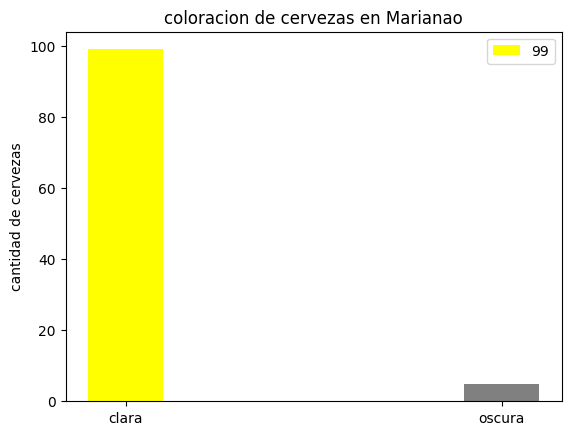
\includegraphics[width=6cm]{c y o.png}
    \caption{Coloración de Cerveza}
    \label{fig:logo}
\end{figure}
Es abismal la diferencia entre una y otra, es casi como si las cervezas oscuras no existieran, y esto se debe más bien a datos geográficos que corresponden con nuestro país. 
Al ser Cuba un país tropical, evidentemente la necesidad del ciudadano cubano es relajar el calor a veces intenso en el que vivimos con cualquier cosa que nos refresque, bueno, ese algo en este caso es la cerveza. 
Está demostrado que la cerveza clara tiene mayor popularidad y es más consumida en el mundo que la cerveza oscura, y Cuba no está lejos de ser parte de eso. 
Con más razón, dada la evidente necesidad del ciudadano residente en Cuba de aminorar un poco y refrescarse, la mayoría opta por beber las cervezas claras por ser más refrescantes y suaves.

\subsection{Cervezas Únicas}
En nuestra base de datos con respecto a la \textbf{Cerveza} podemos ver que existen marcas que tenían una escasez prominente en los locales de venta. 
Precisamente esto nos llevó a preguntarnos: ¿Por qué sucede esto? y ¿Cuáles son estas marcas?.

La siguiente tabla muestra cuáles son estas marcas, junto con las veces en las que se encontró dicha marca en nuestra recolección.
\begin{center}
    \begin{tabular}{|c|c|}
    \hline
    Marca & Cantidad\\
    \hline
    Presidente & 4\\
    \hline
    Martens & 4\\
    \hline
    Bucanero & 3\\
    \hline
    Colonia & 2\\
    \hline
    Covey & 2\\
    \hline
    Shekels & 2\\
    \hline
    Belga Star & 2\\
    \hline
    La Salve & 2\\
    \hline
    Vitalsberg & 1\\
    \hline
    Timber & 1\\
    \hline
    Amstel & 1\\
    \hline
    Patronus & 1\\
    \hline
    Halcón Pelegrino & 1\\
    \hline
    Germania & 1\\
    \hline
    Faxe & 1\\
    \hline
    Corona & 1\\
    \hline
    Beer & 1\\
    \hline
    Zubr & 1\\
    \hline
    \end{tabular}
\end{center}
En el listado encontramos varias marcas y a su lado derecho la cantidad de veces encontradas. 
Esto nos lleva a decir que, por el número de repeticiones, son cervezas que no tienen alta disponibilidad en los locales de venta de esta bebida.

Hay varias razones. 
La primera es principalmente por la dificultad de producción antes vista y esto sucede en el caso de cervezas de Cuba como la Bucanero. 
Su difícil producción limita su disponibilidad, a eso sumarle lo anterior referible a la comparación entre las cervezas claras y oscuras. 
Bucanero, al ser cerveza oscura, su producción es menor debido a la popularidad de las cervezas claras y la unión de estas problemáticas son factores que de una forma u otra afectan la demanda de esta marca y eso se ve reflejado en los datos.

La otra razón es simple, ya que algunas de estas marcas como son la Zubr, Corona, Germania y entre otras forman parte del conjunto de países que aún no tienen gran auge en la exportación de cerveza con Cuba. 
Al ser reducida la entrada al país y bastante limitada, como es de esperar, su disponibilidad será relativa y variada con respecto a los lugares. 
Se priorizarán provinciasy municipios del país con más desenvolvimiento económico, donde será más factible al país recuperar la ganancia. 
Debido a esto, municipios como Marianao son los que van a mediados en la lista, por lo cual provoca una escasez de estas marcas de cerveza.

\subsection{Ubicaciones}
Sobre este tema, fue un dato muy curioso, ya que al analizar las cervezas por su ubicación, nos dimos cuenta de una diferencia que ocurría en la mayoría de las cervezas. 
Marianao tiene varios lugares céntricos, pero ninguno como los hospitales, que es donde hay mayor movimiento de personas cerca de esos lugares, lo que implica que hay mayor movimiento de dinero. 
Dada esta situación, nos dimos cuenta de que en los locales y ubicaciones cerca de estos lugares céntricos, el precio de la cerveza varía, o sea que es mayor en comparación con los lugares alejados de esta ubicación. 
Como demostración de nuestra teoría, tomamos como ejemplo el Hospital Militar de Marianao \textbf{Carlos J. Finlay} y como muestra localidades de venta de cerveza Cristal para hacer esta comparación que le mostramos en el mapa de nuestro proyecto.

Como podemos ver el mapa demuestra nuestra teoria. Existe diferencia entre la venta de cerveza cerca de lugares centricos con respecto a los lugares mas alejados. 
Y esto se debe a lo antes mencionado, mientras mas personas visiten con frecuencias estos lugares es directamente proporcional a la diferencia de precio, no siempre tiene porque ocurrir pero la mayoria de las veces sucedes y esta es la demostración de que existe.
\section{Cebolla}
La cebolla es una hortaliza común en todo el mundo y ha sido utilizada por la humanidad a miles de años. 
Desde la antigüedad, la cebolla ha sido valorada tanto por sus propiedades culinarias como medicinales, y ha sido objeto de estudio en numerosas investigaciones científicas debido a sus posibles beneficios en la salud. 
Y se ha ganado esta vez el lugar de ser analizada e investigada por nosotros. Así que vamos a ver diferentes datos y análisis de este producto.

\subsection{Disponibilidad en el mercado}
La cebolla es un producto que en Cuba podemos verlo y localizarlo igualmente en agros, mercados, puestos e incluso en cualquier vendedor ambulante con una carreta, pero aún así, en el municipio Marianao, nos ha costado encontrarla. 
Así que, teniendo las localizaciones de los lugares donde encontramos cebollas y las que no encontramos, hicimos la comparación por medio de otro mapa de la disponibilidad de la cebolla en el municipio el cual está disponible en nuestro proyecto. 
Sin embargo podemos ver en el siguiente gráfico de pastel el porcentaje de disponibilidad. 

\begin{figure}[h]
    \center
    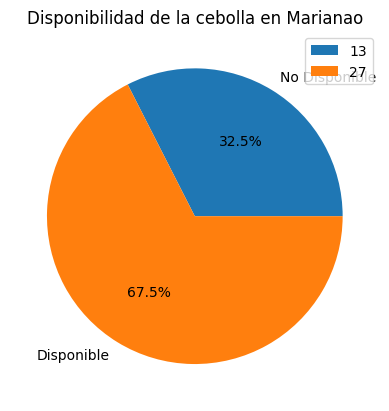
\includegraphics[width=7cm]{disponibilidad.png}
    \caption{Disponibilidad de la cebolla}
    \label{fig:logo}
\end{figure}

Como podemos notar existe mayor porcentaje en el caso de la disponibilidad pero eso no quita que hay un falta considerable 
en este producto.

\subsection{Variedad}
Una vez localizada la disponibilidad del producto, ya podemos hablar de su variedad. 
Como todos sabemos, está presente los dos tipos de cebolla que hay: la \textbf{blanca} y \textbf{morada}. 
Estos dos tipos de cebollas presentan grandes diferencias y analizar esas diferencias es nuestro trabajo. 
Primeramente, nos planteamos la cantidad de cebolla \textbf{blanca} relacionada con la \textbf{morada}. 
Nos preguntábamos ¿Cuál sería la diferencia entre ellas? Y como es natural, tuvimos un resultado. 
Seguido a la respuesta de la interrogante anterior, surgió otra pregunta, la cual tiene como enunciado: ¿Afectará esto al precio?.

\begin{figure}[h]
    \center
    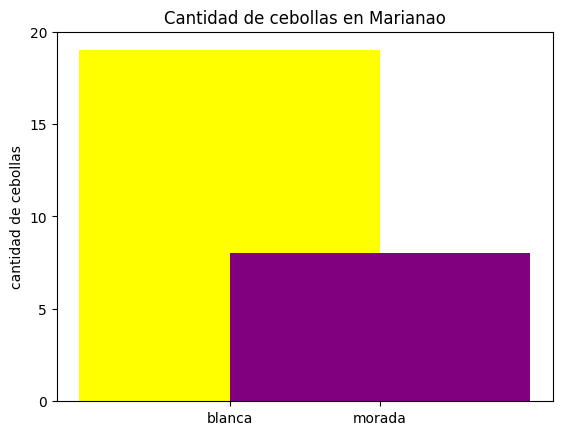
\includegraphics[width=7cm]{variedad.png}
    \caption{Variedad de la cebolla}
    \label{fig:logo}
\end{figure}

Como podemos ver, es considerable la diferencia entre la cebolla \textbf{blanca} y la \textbf{morada}. 
La cebolla \textbf{blanca} va por encima que la \textbf{morada}, y esto es un dato que sobresale y crea otra situación muy interesante que analizar.

A pesar de que ambas cebollas son indispensables en la cocina cubana y no tienen diferencia en su utilización, ya eso quedaría a gusto del consumidor su utilización más frecuente para distintos platos. 
Más allá de que las dos son ricas en vitaminas y minerales esenciales, así como en compuestos antioxidantes y antiinflamatorios que pueden proporcionar beneficios para la salud, y que no presentan mucha diferencia a no ser que una sea más fuerte que otra. 
Pero bueno, el quid de la cosa no está en sus propiedades o sabores, sino en la escasez de una u otra.

Al analizar este dato, nos dimos cuenta de que debido a que hay menos \textbf{cebolla morada} que \textbf{blanca}, la escasez de la \textbf{morada} hace que su precio sea fijo y se mantenga en 200 y, en algún caso, por encima sin ningún tipo de variación, dando lugar a que en los pocos lugares en los que aparezca, su precio será fijo o por encima de lo que se llama normal debido a la escasez que hay. 
Si de por sí hay escasez de cebolla en Marianao, sumarle la escasez de \textbf{cebolla morada}, con razón no se ven variaciones en cuanto a la disminución del precio.

\subsection{Anomalías en el Precio}
Bueno, no queríamos terminar el tema de la cebolla sin antes platicar un poco sobre más que un dato curioso, más bien una exclusividad o rareza en el precio de la cebolla en dos lugares que encontramos en el recorrido realizado para la recolección. 
A continuación, verá dos precios distintos en dos lugares distintos. 
Uno muy excesivo y el otro muy raro por estar por debajo de la norma de aquello que llamamos normal. 
La representación estará dada por ubicaciones en el mapa para que vea el lugar exacto del hecho e incluso se le proporcionará una vía para ver la foto de los lugares si es de su agrado y le da curiosidad ver con sus propios ojos la veracidad de los hechos.
Estará disponible en nuestro proyecto.

\section{Refresco Instantáneo}
\subsection{Zuko}
Zuko es la última incorporación y hay que decir que se ha adueñado de la preferencia gracias a la abundante oferta. 
El auge de Zuko no solo se resume a Cuba, la empresa se ha instaurado en diversos países basando su campaña en la experticia de manufacturar y comercializar bebidas en polvo, escogiendo solo los mejores ingredientes para producirlo.

\subsection{Disponibilidad del Zuko en Cuba}
Zuko es un refresco en polvo que se ha vuelto muy popular en Cuba debido a su sabor delicioso, su facilidad de preparación y su bajo costo en comparación con otros refrescos en el mercado cubano. 
Además, el hecho de que se pueda preparar en casa en cualquier momento lo hace muy atractivo para las familias cubanas. 
Otra razón del auge del refresco Zuko en Cuba es que tiene una amplia variedad de sabores que atraen a los consumidores, como lima, naranja, piña, fresa, melocotón, mango, uva y otros.

También es importante mencionar que la disponibilidad limitada de otros refrescos en la isla ha llevado a muchos consumidores cubanos a buscar otras alternativas de bebidas, como el refresco Zuko. 
Debido a la escasez de productos en Cuba, los consumidores están recurriendo a otras opciones para satisfacer sus necesidades de refrescos y Zuko ha llenado ese vacío de manera efectiva. 
Por lo tanto, su facilidad de preparación, su amplia variedad de sabores y su bajo costo han contribuido al auge del refresco Zuko en Cuba.

Ha habido un aumento significativo en el envío de Zuko a Cuba en losúltimos años. 
El creciente interés por el refresco en la isla ha llevado a fabricantes y distribuidores a aumentar la producción y a enfocar sus esfuerzos en el mercado cubano. 
Además, el hecho de que los consumidores cubanos pueden comprar Zuko en línea ha permitido que sea más accesible para aquellos que no pueden encontrarlo en las tiendas.

También es importante mencionar que el aumento en el envío de Zuko a Cuba está relacionado con el aumento en el turismo en la isla. 
Muchos visitantes de otros países han llevado el gusto por Zuko a Cuba y han creado una demanda adicional para el refresco en la isla. 
Esto ha llevado a una mayor importación de Zuko en Cuba para satisfacer la creciente demanda.

\subsection{Localidades}
Conforme a las localidades en base a la disponibilidad de Zuko, como antes mencionábamos, su popularidad se deja ver a simple vista con su alta disponibilidad en los locales de venta. 
Marianao, como municipio de La Habana, no se queda atrás. Al ser un refresco muy cotizado por la mayoría de las personas, no queda casi ni un lugar en Marianao donde no puedas encontrar un paquetico de este refresco y su gran variedad de sabores.

\section{Refresco Gaseado}
Como último producto en nuestra lista, presentamos el análisis del refresco gaseado o refresco de gas, ya que es una bebida muy popular consumida en todo el mundo. 
Se caracteriza por su burbujeante efervescencia y su sabor dulce y refrescante. Sin embargo, su consumo excesivo ha sido vinculado a una serie de problemas de salud, incluyendo la obesidad, la diabetes y las enfermedades cardíacas. 
El punto es que es un producto interesante a investigar y más allá de las características que pueda tener estaremos haciendo un análisis no distinto a como lo realizamos con los productos anteriores.

Simplemente, la primera pregunta que resalta al investigar este producto sería: ¿Cuáles son las marcas de refresco que se encuentran en el mercado? y ¿Cuáles países las integran?.

Como ya sabemos, Cuba tiene un embargo comercial por el gobierno de Estados Unidos, lo que le imposibilita la importación directa de sus productos de venta y el refresco gaseado está dentro de estos. 
Cuba depende de países terceros para poder realizar este tipo de importaciones al territorio cubano. 
Países como México y Canadá entran en la lista de países donde Cuba accede a la compra de estos productos estadounidenses, y de esta manera es como tenemos variedad de marcas americanas de los refrescos gaseados circulando por nuestro país. 
Representando Estados Unidos el mayor porcentaje de venta de refresco debido a marcas populares como son Pepsi, Coca Cola y Seven Up que hoy se encuentran al por mayor en cafeterías, restaurantes y tiendas de comercialización de productos.

Cuba no se queda atrás y es mayorista en la comercialización de refresco gaseado. No solo exporta, sino que también juega un papel esencial en el consumo y venta de refresco en el país, con la marca Ciego Montero liderando el mayor porcentaje de venta de sodas cubanas en el país. 
En general, losrefrescos y bebidas gaseosas cubanas son populares entre los consumidores en Cuba y se consideran parte de la cultura y la identidad de la isla. 
Tienen una base de consumidores leal y se comercializan como parte de la identidad nacional de Cuba.

Marcas como Santa y Mirinda forman parte del ardor cotidiano de ventas de gaseosas actual. 
Ambas procedentes de España, han cobrado un gran auge en el ámbito cubano. Especializadas principalmente en el sabor naranja, cautivan el paladar de muchas personas en el mundo. 
España entra en la lista de principales países exportadores de refrescos en el mundo, y hoy en día repobla con sus marcas las cafeterías y lugares de ventas en Cuba. 
Junto a Estados Unidos, son el mayor porcentaje de marcas importadas de refrescos vendidas en el país y la gráfica muestra con datos esta relación.

En nuestra lista también tenemos Alemania, que se ha ganado su lugar con la producción de refresco Frisè y la podemos encontrar circulando en nuestro país, aunque no ha ganado mucha popularidad en la región al igual que otras marcas de otros países que se encuentran en la gráfica conformando un número destacable en nuestros datos.

\subsection{Variedad del precio conforme al Envase}
Un dato curioso de analizar es el envase en donde se proporciona el refresco. 
Lo mismo puede ser en una lata que en un pomo, pero ¿Qué tiene de interesante este dato?. 
Mucho, a decir verdad. Aunque no se note, cumple una función bastante significativa al hablar sobre proporciones, precio y también, cómo no, el gusto del público consumidor.

En términos de popularidad y quizás beneficios conforme al envase, se ha estudiado que el mayor porcentaje de venta de refresco en el mundo es de refrescos con envase en lata. 
Ya que, con respecto al sabor, algunos consumidores prefieren los refrescos en lata porque mantiene mucho mejor la frescura y el sabor del producto. 
Esto se debe a que las latas son opacas y no permiten que la luz entre en contacto con el líquido, lo que puede afectar la calidad del sabor con el tiempo. 
Y esto, las grandes empresas productoras de refrescos lo saben. Por esta razón, se puede distinguir una diferencia entre la cantidad de refrescos en latas por encima de las de pomos.

Otro caso a tener en cuenta es la proporción y es evidente en la mayoría de los casos en este tema el volumen en los pomos de refresco es mayor que en las latas. 
Y en temas de gusto, depende de la situación en la que se encuentre el consumidor y la preferencia que desee, conforme a que si quiere más o menos líquido a tomar. 
Pero este dato, además de ser evidente a simple vista, tiene efecto en otro campo, el precio. Este dato influye principalmente en el precio del refresco. 
Al tener mayores volúmenes de líquido, evidentemente su costo será relativamente mayor y esto se puede evidenciar en la gráfica de nuestro proyecto donde se puede analizar cómo la diferencia de refresco en lata es excesiva por encima de la de pomo y por marca, y cómo esto puede influenciar en el precio del refresco.

\subsection{Precios, Marcas y sobre todo Sabor}
Aquí es donde entramos en la variedad de sabores de cada marca vendida en Cuba, como dato interesante en nuestro análisis.

La gráfica interactiva en nuestro proyecto contiene la relación por sabores en las marcas y el precio correspondiente. 
De esta gráfica, podemos sacar mucha información importante y respuestas a preguntas que queramos hacernos referente a este tema. 
Por ejemplo, ¿Cuál es la marca más cara y de qué sabor es? Y sencillamente encontraremos la respuesta evidente de que es la marca Ciego Montero, procedente de Cuba, con sabor a cola y un precio de 400 pesos, y su precio se debe a que su contenido es en envase. 
Podríamos hacernos la pregunta de ¿Cuál es el sabor más predominante? Y veremos cómo la naranja predomina más que la cola o limón. 
Recuérdese que esto está basado en los datos extraídos en el municipio de Marianao. Y con respecto a las marcas, podría surgir la pregunta de ¿Cuál sería la que más abunda? y ¿Cuál es la que más variedad de sabores tiene? 
Respectivamente, la respuesta sería en ambas la Ciego Montero nuevamente.

Puede realizarse cualquier tipo de análisis relacionadosobre este tema basándonos en los datos que nos proporciona la gráfica. 
Y es muy interesante toda la información que podemos sacar de todo esto.

\section{Conclusiones}
Con este último análisis, podemos concluir nuestra presentación de los análisis extraídos sobre los productos cerveza, cebolla, refresco gaseado y refresco instantáneo. 
Hemos trabajado en base a presentar la información lo más explicativa y fácil de disolver para el lector. Basándonos en el análisis que nos pareció interesante debatir y presenciar, esto no quiere decir que sea lo único y exclusivo que se pueda sacar de esta información. 
Estamos abiertos a seguir mejorando y perfeccionando nuestro proyecto. ¿En qué otras preguntas podemos resolver y qué otros datos interesantes podemos sacar de toda esta información?. 
Sin más preámbulos, aquí concluye la presentación. Esperamos que le haya gustado y le haya servido de mucha ayuda para su saber propio.

Muchas gracias.


\newpage
\tableofcontents

\newpage
\bibliography{bibliography}
\end{document}
